%% LaTeX-Beamer template for KIT design
%% by Erik Burger, Christian Hammer
%% title picture by Klaus Krogmann
%%
%% version 2.1
%%
%% mostly compatible to KIT corporate design v2.0
%% http://intranet.kit.edu/gestaltungsrichtlinien.php
%%
%% Problems, bugs and comments to
%% burger@kit.edu

\documentclass[18pt]{beamer}

%% SLIDE FORMAT

% use 'beamerthemekit' for standard 4:3 ratio
% for widescreen slides (16:9), use 'beamerthemekitwide'

\usepackage{templates/beamerthemekit}
% \usepackage{templates/beamerthemekitwide}
\usepackage{graphicx}
\usepackage{csquotes}
%% TITLE PICTURE

% if a custom picture is to be used on the title page, copy it into the 'logos'
% directory, in the line below, replace 'mypicture' with the 
% filename (without extension) and uncomment the following line
% (picture proportions: 63 : 20 for standard, 169 : 40 for wide
% *.eps format if you use latex+dvips+ps2pdf, 
% *.jpg/*.png/*.pdf if you use pdflatex)

%\titleimage{mypicture}

%% TITLE LOGO

% for a custom logo on the front page, copy your file into the 'logos'
% directory, insert the filename in the line below and uncomment it

%\titlelogo{mylogo}

% (*.eps format if you use latex+dvips+ps2pdf,
% *.jpg/*.png/*.pdf if you use pdflatex)

%% TikZ INTEGRATION

% use these packages for PCM symbols and UML classes
\usepackage{templates/tikzkit}
\usepackage{templates/tikzuml}
\usepackage{amsmath}
\usepackage[ruled]{algorithm2e}

% the presentation starts here

\title[Graphen 3]{ICPC}
\subtitle{Graphen 3}
\author{Tobias, Julian, Jakob, Tobias}

\institute{ITI Wagner, IPD Tichy}

% Bibliography

\usepackage[citestyle=authoryear,bibstyle=numeric,hyperref,backend=biber]{biblatex}
\addbibresource{templates/example.bib}
\bibhang1em

\SetKwRepeat{Do}{do}{while}
\SetKwProg{Fn}{Function}{}{}


\begin{document}
	
	% change the following line to "ngerman" for German style date and logos
	\selectlanguage{ngerman}
	
	%title page
	\begin{frame}
	\titlepage
\end{frame}

%table of contents
\begin{frame}{Outline/Gliederung}
\tableofcontents
\end{frame}

\section{Tobias}
\begin{frame}{Einf\"uhrung}
	\begin{figure}
		\centering
		\begin{tikzpicture}[node distance=2cm, auto, thick]
		
			
			\only<1>{\node[state] (s) {$q_1$};
				\node[state, above right = of s] (q0) {$q_0$};
				\node[state, below right = of s] (q1) {$q_3$};
				\node[state, below right = of q0] (t) {$q_2$};}
			
			\visible<2->{\node[state] (s) {$q_0$};
				\node[state, above right = of s, fill=lightgray] (q0) {$s$};
				\node[state, below right = of s, fill=lightgray] (q1) {$t$};
				\node[state, below right = of q0] (t) {$q_1$};}
			
			\path 
				(q0) edge[->,bend left = -20, left] node {30} (s)
				(s) edge[->,bend left = -20, left] node {70} (q1)
				%(q0) edge[->,bend left = 10] node {5} (q1)
				(q0) edge[->,bend right = -20, right] node {60} (t)
				(t) edge[->,bend right = -20, right] node {25} (q1);
			\visible<3-8>{
				\path(q0) edge[->, bend left = 20, red] node {30} (s);}
			\visible<4-8>{
				\path(s) edge[->, bend left = 20, red] node {30} (q1);}
			\visible<5->{
				\path(q0) edge[->, dashed,out=180, in=180, looseness=2, red, left] node {30} (q1);}
			\visible<6-8>{
				\path(q0) edge[->, bend right = 30, red] node {60} (t);}
			\visible<7-8>{
				\path(t) edge[->, bend right = 30, red] node {25} (q1);}
			\visible<8->{
				\path(q0) edge[->, dashed,out = 0, in = 0, looseness = 2, red, right] node {25} (q1);}
			\visible<9->{
				\path (t) edge[->, bend right = 10, black, above left] node {60} (s);}
			\only<10>{
				\path
				(q0) edge[->, bend right = 10,  red, right] node {} (t)
				(t) edge[->, bend left = 10,  red] node {} (s)
				(s) edge[->, bend left = 10, red, right] node {} (q1);}
			\visible<11->{
				\path
				(q0) edge[->, bend right = 10,  red, right] node {35} (t)
				(t) edge[->, bend left = 10,  red, below left] node {60} (s)
				(s) edge[->, bend left = 10, red, right] node {40} (q1);}
			\visible<12->{
				\path (q0) edge[->, dashed, red] node {35} (q1);}
			
		\end{tikzpicture}		
	\end{figure}
	
	\centering
	\only<1>{Gegeben gerichteter Graph}
	\only<2>{s: source, t:sink}
	\only<3>{Fluss}
	\only<4>{Flusserhaltung} 
	\only<5>{Wert eines s-t-Flusses}
	\only<11>{Exzess: Werte entsprechend der Kantenkapazit\"at abz\"uglich bereits vorhandener Fl\"usse}
\end{frame}

\begin{frame}{Flussprobleme}
	\begin{itemize}
		\visible<1->{\item Schwierigeit im Erkennen der Aufgaben}
		\only<1>{\item[\,]Proble UVa xxx} % TD bspl aufgabe
		\visible<2->{\item Seit 2013 vermehrtes vorkommen in contests}
		\only<2>{\item[] decider Problem}
	\end{itemize}
\end{frame}

\section{Max-Flow Algorithmen}
\begin{frame}{Bestimmung des maximalen Flusses}
Idee:
\begin{itemize}
	\item Starte mit dem leeren Fluss
	\item Bestimme erweiternden Pfad (augmenting path) P, auf dem der Fluss von s nach t vergr\"o{\ss}erbar ist
	\item Erweitere die L\"osung um Pfad P
	\item Wiederhole so oft, wie es einen passenden Pfad P gibt
\end{itemize}
Frage: Wie kann P gefunden werden?
\end{frame}

\subsection{Ford-Fulkerson}
\begin{frame}{Ford-Fulkerson Algorithmus}
\begin{itemize}
	\item Greedy Algorithmus ver\"offentlicht in 1956 von L. R. Ford, Jr. und D. R. Fulkerson
	\item Verwendet Tiefensuche um den erweiternden Pfad P zu bestimmen
	\item Die L\"osung wird um P erweitert indem, 
	\begin{itemize}
		\item die geringste Kapazit\"at f einer Kante in P bestimmt wird
		\item die Kapazit\"aten aller Kanten in P um f verringert werden
		\item die Kapazit\"aten aller Gegenkanten um f erh\"oht werden
		\item der maximale Fluss um f erh\"oht wird
	\end{itemize}  
\end{itemize}
\end{frame}

\begin{frame}{Ford-Fulkerson Algorithmus}
\begin{figure}
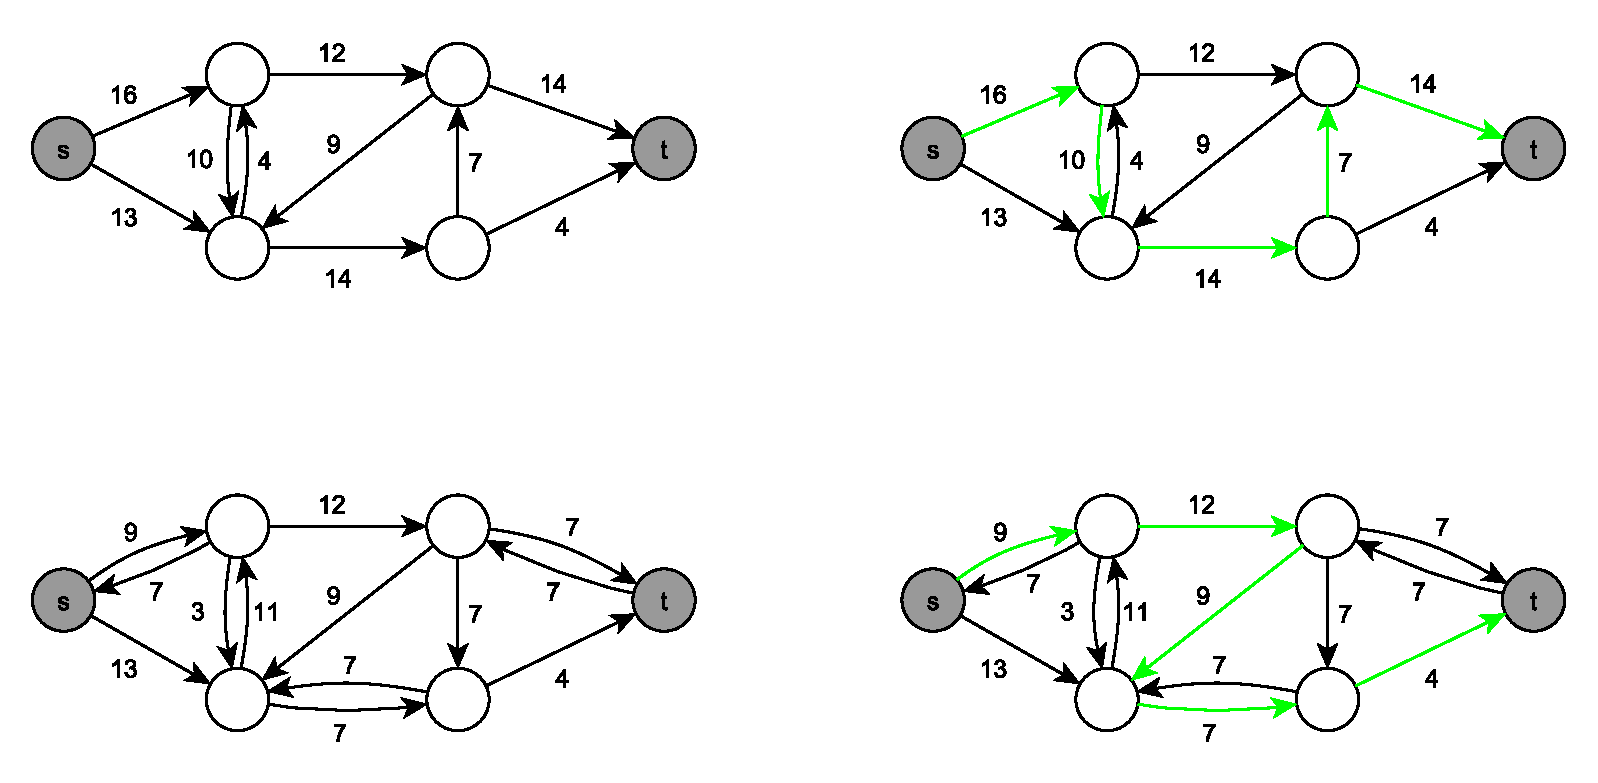
\includegraphics[width = \textwidth]{img/Jakob_Ford.pdf}
\end{figure}
\end{frame}


\begin{frame}{Ford-Fulkerson Algorithmus}
\begin{figure}
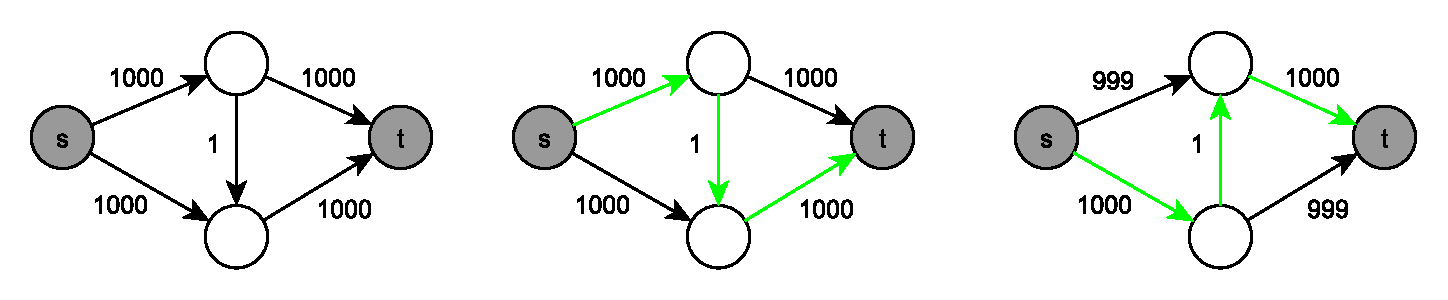
\includegraphics[width = \textwidth]{img/Jakob_Ford2.pdf}
\end{figure}
\begin{itemize}
	\item Im Worst-Case wird der maximale Fluss pro Iteration nur um 1 erh\"oht
	\item[$\Rightarrow$]  Laufzeit in $\mathcal O(|f^*|\cdot |E|)$, wobei $|f^*|$ der Wert des maximalen Flusses beschreibt
	\item Deshalb \textbf{nicht} f\"ur ICPC-Aufgaben geeignet!
\end{itemize}
\end{frame}

\subsection{Edmonds-Karp}
\begin{frame}{Edmonds-Karp Algorithmus}
\begin{itemize}
\item 1972 von J. Edmonds und R. M. Karp ver\"offentlicht
\item Verwendet Breitensuche um den k\"urzesten erweiternden Pfad P zu bestimmen
\item Erweiterung der L\"osung um P analog zu Ford-Fulkerson
\item Die L\"ange des erweiternden Pfades ist monoton steigend
\item Es sind maximal $|V|\cdot |E|$ Iterationen notwendig
\item[$\Rightarrow$] Laufzeit in $\mathcal O(|V| \cdot |E|^2)$
\end{itemize}
\end{frame}

\begin{frame}{Edmonds-Karp Implementierung}
\SetEndCharOfAlgoLine{}
\begin{algorithm}[H]
	\Fn{Max-Flow (G = (V, E), s, t, c)}{
		$maxFlow = 0 $ \;
		\Do{P exists}{
			find augmenting path P using BFS\;
			$ f = min (c(u,v) | (u,v) \in P)$\;
			\ForEach{$(u,v) \in P$}{
				 c(u,v) -= f  \;
				 c(v,u) += f  \;
			}
			maxFlow += f \;
		}
		\textbf{return} maxFlow \;
	}
	\caption{Edmonds-Karp}
\end{algorithm}
\end{frame}

\begin{frame}{Edmonds-Karp Algorithmus}
\begin{figure}
	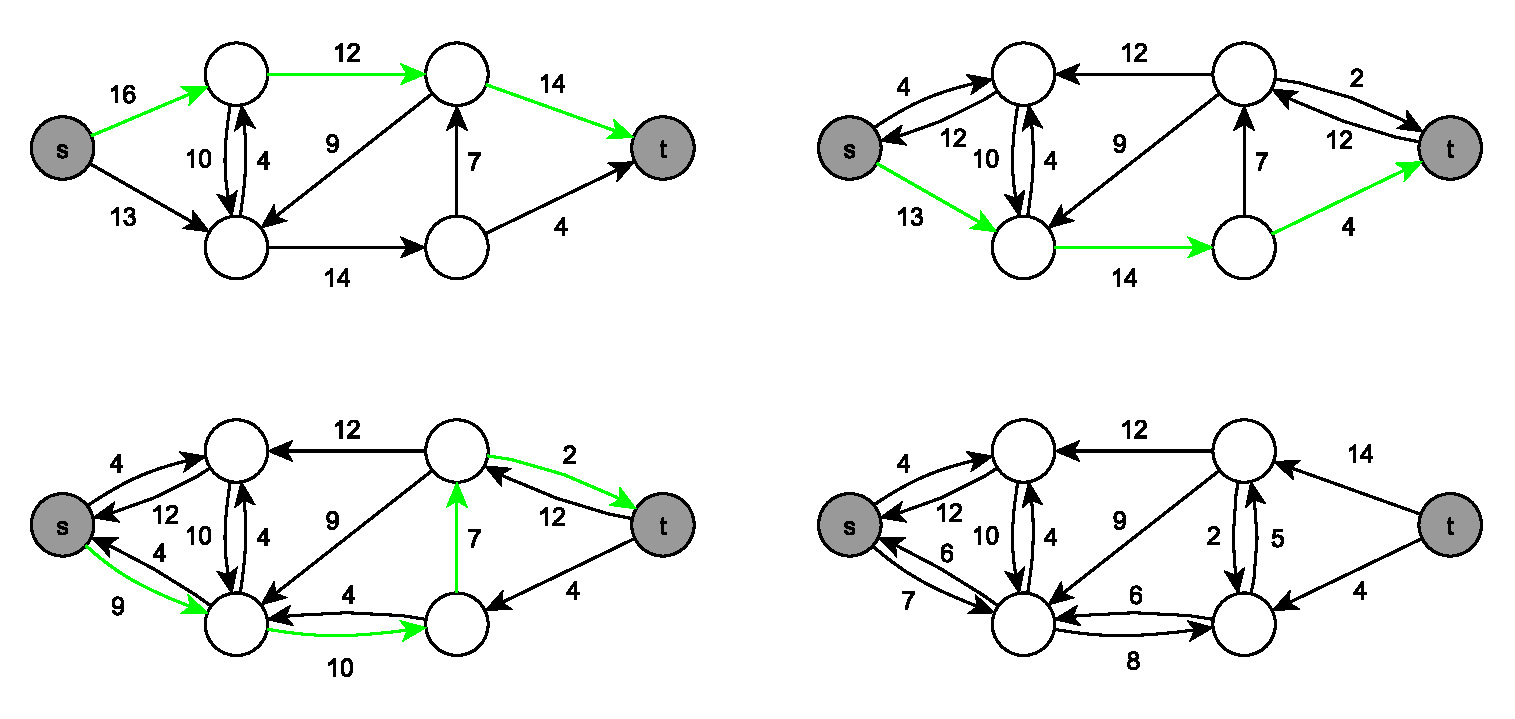
\includegraphics[width = \textwidth]{img/Jakob_Edmond.pdf}
\end{figure}
\end{frame}

\begin{frame}{Edmonds-Karp Implementierungsdetails}
\begin{itemize}
	\item In Adjazenzliste neben Zielknoten auch Kapazit\"at und Verweis auf die R\"uckkante speichern
	\item In Breitensuche nur Kanten mit positiver Kapazit\"at ber\"ucksichtigen
	\item Breitensuche abbrechen, sobald t erreicht wurde
\end{itemize}
\end{frame}


\section{Julian}
\begin{frame}{Min-Cut}
\begin{block}{Min-Cut}

\begin{itemize}
\item Definiere Schnitt \(C = (S-Komponente, T-Komponente)\) als Partition von \(V \in G \), wobei \(s \in S-Komponente\) und \(t \in T-Komponente\) 
\item Weiter sei die Schnittmenge \(c = \{(u, v) \in E | u \in S-Komponente \land v \in T-Komponente\}\)
\item W\"ahle \(c\) so, dass Max Flow von \(s\) nach \(t\) 0 ist, f\"ur \(E'=E\setminus c\) 
\end{itemize}
\end{block}
\end{frame}

\begin{frame}{Max-Flow-Min-Cut-Theorem}
\begin{block}{Max-Flow-Min-Cut-Theorem}
\begin{itemize}
\item Ein maximaler Fluss im Netzwerk hat genau den Wert eines minimalen Schnitts.
\end{itemize}
\end{block}
\end{frame}

\begin{frame}{Max-Flow-Min-Cut}
\begin{itemize}
\item Bsp.:
\end{itemize}
\begin{center}
\begin{tikzpicture}[node distance=2cm, auto, thick]
\node[state, fill=lightgray] (s) {$s$};
\node[state, right=of s] (q0) {$q_0$};
\node[state, below=of s] (q1) {$q_1$};
\node[state, below=of q0, fill=lightgray] (t) {$t$};

\path (s) edge[->,bend left = 10] node {30} (q0)
(s) edge[->,bend left = 10] node {70} (q1)
(q0) edge[->,bend left = 10] node {30} (s)
(q0) edge[->,bend left = 10] node {5} (q1)
(q0) edge[->,bend left = 10] node {70} (t)
(q1) edge[->,bend left = 10] node {70} (s)
(q1) edge[->,bend left = 10] node {5} (q0)
(q1) edge[->,bend left = 10] node {25} (t)
(t) edge[->,bend left = 10] node {70} (q0)
(t) edge[->,bend left = 10] node {25} (q1);
\end{tikzpicture}
\begin{tikzpicture}[node distance=2cm, auto, thick]
\node[state, fill=lightgray] (s) {$s$};
\node[state, right=of s] (q0) {$q_0$};
\node[state, below=of s] (q1) {$q_1$};
\node[state, below=of q0, fill=lightgray] (t) {$t$};

\path (s) edge[->,bend left = 10, dashed, color=blue] node {0} (q0)
(s) edge[->,bend left = 10, dashed] node {40} (q1)
(q0) edge[->,bend left = 10] node {60} (s)
(q0) edge[->,bend left = 10] node {10} (q1)
(q0) edge[->,bend left = 10, dashed] node {35} 	(t)
(q1) edge[->,bend left = 10] node {100} (s)
(q1) edge[->,bend left = 10, dashed, color=blue] node {0} (q0)
(q1) edge[->,bend left = 10, dashed, color=blue] node {0} (t)
(t) edge[->,bend left = 10] node {105} (q0)
(t) edge[->,bend left = 10] node {50} (q1);
\end{tikzpicture}
\end{center}
\begin{itemize}
\item Hier
\begin{itemize}
\item \(C=(\{s,q_1\}, \{t, q_0\})\)
\item \(c=\{(s,q_0), (q_1,q_0), (q_1, t)\}\) 
\end{itemize} 
\end{itemize}
\end{frame}

\begin{frame}{Multi-Quelle/Multi-Abfluss}
\begin{itemize}
\item Gegeben sei folgende Situation:
\end{itemize}
\begin{center}
\begin{tikzpicture}[auto, thick]
\node[state, fill=lightgray] (s1) {$s$};
\node[state, below=of s, fill=lightgray] (s2) {$s$};
\node[state] (q1) at (2,-1) {};
\node[state, fill=lightgray] (t1) at (4,0) {$t$};
\node[state, below=of t1, fill=lightgray] (t2) {$t$};

\path (s1) edge[->] node {} (q1)
(s2) edge[->] node {} (q1)
(q1) edge[->] node {} (t1)
(q1) edge[->] node {} (t2);
\end{tikzpicture}
\end{center}
\begin{itemize}
\item Problem: Max-Flow Algorithmus kann nur mit einer Quelle und einer Senke arbeiten.
\item L\"osung: Ertelle Super-Quelle und Super-Senke und verbinde alle Quellen und Senken mit Kantengewicht $\infty$
\end{itemize}
\end{frame}

\begin{frame}{Multi-Quelle/Multi-Abfluss L\"osung}
\begin{center}
\begin{tikzpicture}[auto, thick]
\node[state, fill=lightgray] (ss) at (-2,-1) {$ss$};
\node[state] (s1) {$s$};
\node[state, below=of s] (s2) {$s$};
\node[state] (q1) at (2,-1) {};
\node[state] (t1) at (4,0) {$t$};
\node[state, below=of t1] (t2) {$t$};
\node[state, fill=lightgray] (st) at (6, -1) {$st$};

\path (s1) edge[->] node {} (q1)
(s2) edge[->] node {} (q1)
(q1) edge[->] node {} (t1)
(q1) edge[->] node {} (t2)
(ss) edge[->] node {$\infty$} (s1)
(ss) edge[->] node {$\infty$} (s2)
(t1) edge[->] node {$\infty$} (st)
(t2) edge[->] node {$\infty$} (st);
\end{tikzpicture}
\end{center}
\end{frame}


\begin{frame}{Knotenkapazit\"at}
\begin{itemize}
\item Gegeben sind Knoten mit Kapazit\"at.
\item Bsp.:
\end{itemize}
\begin{center}
\begin{tikzpicture}[auto, thick]
\node[state] (V) {$V|7$};

\path (V) edge[->] node {5} (1.5,0)
(-1, 1) edge[->] node {10} (V)
(-1, -1) edge[->] node {4} (V);
\end{tikzpicture}
\end{center}
\end{frame}

\begin{frame}{Knotenkapazit\"at}
\begin{itemize}
\item Gegeben sind Knoten mit Kapazit\"at.
\item Bsp.:
\end{itemize}
\begin{center}
\begin{tikzpicture}[auto, thick]
\node[state] (V1) {$V_{in}$};
\node[state, right=of V1] (V2) {$V_{out}$};

\path (V1) edge[->] node {7} (V2)
(-1, 1) edge[->] node {10} (V1)
(-1, -1) edge[->] node {4} (V1)
(V2) edge[->] node {5} (3.5, 0);
\end{tikzpicture}
\end{center}
\end{frame}

\begin{frame}{Modellierung}
\begin{itemize}
\item Erkennen eines Netzwerkfluss-Problems nicht immer einfach
\pause
\item Was hilft?
\begin{itemize}
\pause
\item \"Ubung
\item \"Ubung
\item ...
\end{itemize}
\end{itemize}
\end{frame}

\begin{frame}{Modellierung - Beispiel}
\begin{itemize}
\item Situation: Die Titanic ist gesunken. Es soll ermittelt werden wie viele Menschen gerettet werden k\"onnen.
\item Eingabe: X, Y, P mit X,Y Dimension der Fl\"ache (\(1 \leq X,Y \leq 30\)) und P (\(P \leq 10\)) die Anzahl von Personen, welche gleichzeitig auf ein Holzbrett k\"onnen.
\end{itemize}
\begin{center}
\begin{tabular}{c|l}
Symbol & Bedeutung \\
\hline
* & Menschen auf Treibeis \\
\(\sim\) & Eiskaltes Wasser \\
. & Treibeis \\
@ & Gro\ss er Eisberg \\
\# & Gro\ss es Holzbrett \\
\end{tabular}
\end{center}
\end{frame}

\begin{frame}{Modellierung - Beispiel}
\begin{itemize}
\item Gegeben sei nun folgende Eingabe:
\end{itemize}
\begin{center}
\begin{tabular}{cccc}
* & \(\sim\) & \(\sim\) & \# \\
. & . & . & @ \\
. & \(\sim\) & . & * \\
\end{tabular}
\end{center}
\begin{itemize}
\pause\item Wandle in Graphen um...
\end{itemize}
\end{frame}

\begin{frame}{Modellierung - Beispiel}
\begin{center}
\begin{tikzpicture}[auto, thick]
\node[state] (1) {$*$};
\node[state, right=of 1] (2) {\(\sim\)};
\node[state, right=of 2] (3) {\(\sim\)};
\node[state, right=of 3] (4) {\#};
\node[state, below=of 1] (5) {$.$};
\node[state, right=of 5] (6) {$.$};
\node[state, right=of 6] (7) {$.$};
\node[state, right=of 7] (8) {@};
\node[state, below=of 5] (9) {$.$};
\node[state, right=of 9] (10) {\(\sim\)};
\node[state, right=of 10] (11) {$.$};
\node[state, right=of 11] (12) {$*$};
\end{tikzpicture}
\end{center}
\begin{itemize}
\pause
\item Verbinde alle Knoten, \"uber die ein Weg m\"oglich ist...
\end{itemize}
\end{frame}

\begin{frame}{Modellierung - Beispiel}
\begin{center}
\begin{tikzpicture}[auto, thick]
\node[state] (1) {$*$};
\node[state, right=of 1] (2) {\(\sim\)};
\node[state, right=of 2] (3) {\(\sim\)};
\node[state, right=of 3] (4) {\#};
\node[state, below=of 1] (5) {$.$};
\node[state, right=of 5] (6) {$.$};
\node[state, right=of 6] (7) {$.$};
\node[state, right=of 7] (8) {@};
\node[state, below=of 5] (9) {$.$};
\node[state, right=of 9] (10) {\(\sim\)};
\node[state, right=of 10] (11) {$.$};
\node[state, right=of 11] (12) {$*$};

\path (1) edge[-] node {} (5)
(5) edge[-] node {} (6)
(5) edge[-] node {} (9)
(6) edge[-] node {} (7)
(7) edge[-] node {} (8)
(7) edge[-] node {} (11)
(8) edge[-] node {} (4)
(8) edge[-] node {} (12);
\end{tikzpicture}
\end{center}
\begin{itemize}
\pause
\item F\"uge Knotengewichte hinzu...
\end{itemize}
\end{frame}

\begin{frame}{Modellierung - Beispiel}
\begin{center}
\begin{tikzpicture}[auto, thick]
\node[state] (1) {$*|1$};
\node[state, right=of 1] (2) {\(\sim\)};
\node[state, right=of 2] (3) {\(\sim\)};
\node[state, right=of 3] (4) {\# $|1000$};
\node[state, below=of 1] (5) {$.|1$};
\node[state, right=of 5] (6) {$.|1$};
\node[state, right=of 6] (7) {$.|1$};
\node[state, right=of 7] (8) {@$|1000$};
\node[state, below=of 5] (9) {$.|1$};
\node[state, right=of 9] (10) {\(\sim\)};
\node[state, right=of 10] (11) {$.|1$};
\node[state, right=of 11] (12) {$*|1$};

\path (1) edge[-] node {} (5)
(5) edge[-] node {} (6)
(5) edge[-] node {} (9)
(6) edge[-] node {} (7)
(7) edge[-] node {} (8)
(7) edge[-] node {} (11)
(8) edge[-] node {} (4)
(8) edge[-] node {} (12);
\end{tikzpicture}
\end{center}
\begin{itemize}
\pause
\item Verbinde alle Menschen mit s und alle Holzbretter mit t...
\end{itemize}
\end{frame}

\begin{frame}{Modellierung - Beispiel}
\begin{center}
\begin{tikzpicture}[auto, thick]
\node[state] (1) {$*|1$};
\node[state, right=of 1] (2) {\(\sim\)};
\node[state, right=of 2] (3) {\(\sim\)};
\node[state, right=of 3] (4) {\# $|1000$};
\node[state, below=of 1] (5) {$.|1$};
\node[state, right=of 5] (6) {$.|1$};
\node[state, right=of 6] (7) {$.|1$};
\node[state, right=of 7] (8) {@$|1000$};
\node[state, below=of 5] (9) {$.|1$};
\node[state, right=of 9] (10) {\(\sim\)};
\node[state, right=of 10] (11) {$.|1$};
\node[state, right=of 11] (12) {$*|1$};

\path (1) edge[-] node {} (5)
(5) edge[-] node {} (6)
(5) edge[-] node {} (9)
(6) edge[-] node {} (7)
(7) edge[-] node {} (8)
(7) edge[-] node {} (11)
(8) edge[-] node {} (4)
(8) edge[-] node {} (12);

\node[state, left=of 5] (s) {$s$};
\node[state, right=of 8] (t) {$t$};

\path (s) edge[->] node {1} (1)
(s) edge[->] node {1} (12)
(4) edge[->] node {P} (t);
\end{tikzpicture}
\end{center}
\begin{itemize}
\item Bem.: Knotengewichte m\"ussen noch aufgel\"ost werden
\end{itemize}
\end{frame}

\section{Tobias T}
\begin{frame}{Bipartiter Graph}
\begin{itemize}
\item Bipartiter Graph
\end{itemize}
\begin{figure}
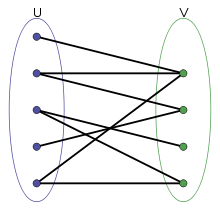
\includegraphics[width = 0.5\textwidth] {img/TobiasT_Bipartit.jpg}
\end{figure}
\end{frame}

\begin{frame}{Matching}
\begin{itemize}
\item Definitionen: Matching, maximales Matching, kardinalit\"atsmaximales Matching, perfektes Matching
\end{itemize}
\begin{figure}
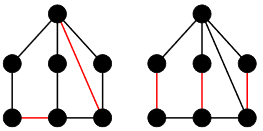
\includegraphics[width = 0.5\textwidth]{img/TobiasT_Matching.jpg}
\end{figure}
\end{frame}


\begin{frame}{Laufzeit}
\begin{itemize}
\item Kurz auf Laufzeit eingehen
\item Beispiel: Primzahlen (Competitive Programming 3, Seite 180)
\item Definitionen: Max Independent Set, Min Vertex Cover, K\"onigs‘ Theorem: |Min Vertex Cover| = |größtes Matching|
\end{itemize}
\begin{figure}
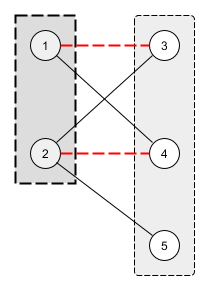
\includegraphics[width = 0.2\textwidth] {img/TobiasT_Laufzeit.jpg}
\end{figure}
\end{frame}

\begin{frame}{Modelierung}
\begin{itemize}
\item Beispiel: Guardian of Decency (Competitive Programming 3, Seite 182)
\item (Je nach verbleibender Zeit:) noch mehr Graphentheorie: bipartit $< == >$ keine ungeraden Kreise, ...
\end{itemize}
\end{frame}

\end{document}
